%% ============================================================
%% LECCIÓN 1.2: LÍMITES, CONTINUIDAD Y DERIVADAS PARCIALES
%% Cálculo III — UIS (20254)
%% Contenido basado en LPS_L1.2.pdf y Constitución de lecciones
%% Estilo: Apostol unificado, con entornos LaTeX personalizados
%% ============================================================

\chapter{Límites, Continuidad y Derivadas Parciales}

La teoría de funciones de una variable nos enseñó que el comportamiento
de una función cerca de un punto se captura mediante el límite, y que
la regularidad de ese comportamiento se expresa con la continuidad.
También aprendimos que la razón de cambio instantánea de una función
es la derivada. En esta lección extenderemos estas tres nociones
fundamentales —límite, continuidad y derivada— a funciones de dos o
más variables. La extensión no es meramente formal: el hecho de que
el dominio sea ahora un espacio de dimensión superior introduce una
novedad cualitativa: el punto de aproximación puede alcanzarse a lo
largo de infinitas trayectorias distintas. En una variable solo hay
dos direcciones (izquierda y derecha); en dos variables hay infinitas
curvas que convergen al mismo punto, y la existencia del límite exige
que el valor límite sea el mismo a lo largo de \emph{todas} ellas.

\begin{rem}
El hilo conductor de esta lección es el siguiente principio: para
funciones de varias variables, todo concepto que dependa de la
``proximidad'' se formula en términos de la \textbf{distancia
euclidiana} entre puntos. El límite exige que la función se acerque a
un valor $L$ cuando la distancia entre $(x,y)$ y $(a,b)$ tiende a cero,
\emph{independientemente de la dirección desde la que se aproxime}.
Esta independencia direccional es la novedad central y la principal
fuente de dificultad.
\end{rem}

% ============================================================
% SECCIÓN 1.3: LÍMITE Y CONTINUIDAD DE UNA FUNCIÓN DE VARIAS VARIABLES
% ============================================================

\section{Límite y continuidad de una función de varias variables}

Empezamos con el concepto de límite para funciones de dos variables,
que luego extenderemos a tres o más.

\begin{definition}[Límite de una función de dos variables]
Sea $f$ una función definida en un disco abierto centrado en $(a,b)$,
excepto posiblemente en $(a,b)$. Decimos que
\[
\lim_{(x,y)\to(a,b)} f(x,y) = L
\]
si para todo $\varepsilon>0$ existe $\delta>0$ tal que
\[
0 < \sqrt{(x-a)^2 + (y-b)^2} < \delta
\quad\Longrightarrow\quad
|f(x,y)-L| < \varepsilon.
\]
\end{definition}

Esta definición es la análoga bidimensional de la definición
$\varepsilon$-$\delta$ para una variable: la distancia entre $(x,y)$ y
$(a,b)$ se mide ahora con la norma euclidiana en $\mathbb{R}^2$, y
la condición $0<\sqrt{\cdots}$ excluye al punto $(a,b)$ del análisis,
pues el límite no depende del valor de $f$ en ese punto.

\begin{rem}
La definición exige que la función esté definida en \emph{algún}
disco perforado alrededor de $(a,b)$; no necesita estar definida
exactamente en $(a,b)$. Esta es la misma convención que en una
variable.
\end{rem}

\begin{rem}
Para funciones de tres variables, la definición es idéntica
sustituyendo la distancia en $\mathbb{R}^3$:
\[
\lim_{(x,y,z)\to(a,b,c)} f(x,y,z) = L
\]
si para todo $\varepsilon>0$ existe $\delta>0$ tal que
$0<\sqrt{(x-a)^2+(y-b)^2+(z-c)^2}<\delta$ implica
$|f(x,y,z)-L|<\varepsilon$.
\end{rem}

La diferencia fundamental con el caso unidimensional es que ahora el
punto $(a,b)$ puede ser alcanzado por \emph{infinitas trayectorias}
distintas en el plano. En una variable, solo hay dos caminos de
aproximación: por la izquierda o por la derecha. En dos variables,
hay infinitos: rectas de cualquier pendiente, curvas como parábolas,
cúbicas, etc., que pasen por $(a,b)$. Para que el límite exista, el
valor de $f$ debe tender al mismo $L$ a lo largo de \emph{todas}
ellas. Si encontramos dos trayectorias que producen valores límite
distintos, el límite no existe.

\begin{rem}
Este principio es análogo al de los límites laterales en una variable:
$\lim_{x\to a}f(x)$ existe si y solo si $\lim_{x\to a^-}f(x)$ y
$\lim_{x\to a^+}f(x)$ existen y coinciden. En varias variables, los
límites laterales se reemplazan por límites a lo largo de trayectorias,
y hay infinitas trayectorias posibles.
\end{rem}

\begin{pasos}[Para determinar si un límite de dos variables existe]
\begin{enumerate}
    \item \textbf{Prueba de trayectorias.} Si la función es sencilla,
    intentar evaluar a lo largo de rectas $y=mx$ (o curvas $y=x^2$,
    $x=y^2$, etc.) que pasen por el punto. Si dos trayectorias
    conducen a valores distintos, el límite no existe.
    \item \textbf{Sustitución directa.} Si la función es continua en el
    punto (por ejemplo, polinómica), el límite es $f(a,b)$.
    \item \textbf{Manipulación algebraica.} Factorizar, racionalizar o
    simplificar para eliminar indeterminaciones.
    \item \textbf{Coordenadas polares.} Si el punto de aproximación es
    el origen, usar $x=r\cos\theta$, $y=r\sin\theta$. Si el límite
    cuando $r\to 0$ es independiente de $\theta$, el límite existe; si
    depende de $\theta$, no existe.
    \item \textbf{Teorema del emparedado.} Acotar $|f(x,y)-L|$ por
    una función que tiende a cero.
\end{enumerate}
\end{pasos}

\begin{example}[Límite que no existe por trayectorias distintas]
Sea
\[
f(x,y) = \frac{x^2 y}{x^4 + y^2}.
\]
Estudiar $\lim_{(x,y)\to(0,0)} f(x,y)$.
\end{example}

\begin{myproof}
\textbf{Paso 1. Prueba de trayectorias.} Evaluamos a lo largo de dos
trayectorias distintas que pasan por el origen.

\textit{Trayectoria 1:} $y=x$. Entonces
\[
f(x,x) = \frac{x^2\cdot x}{x^4+x^2} = \frac{x^3}{x^2(x^2+1)}
        = \frac{x}{x^2+1}.
\]
Cuando $x\to 0$,
\[
\lim_{x\to 0} \frac{x}{x^2+1} = 0.
\]

\textit{Trayectoria 2:} $y=x^2$. Entonces
\[
f(x,x^2) = \frac{x^2\cdot x^2}{x^4+(x^2)^2}
          = \frac{x^4}{x^4+x^4} = \frac{1}{2}.
\]
Cuando $x\to 0$,
\[
\lim_{x\to 0} \frac{1}{2} = \frac{1}{2}.
\]

\textbf{Conclusión.} Como las dos trayectorias producen límites
distintos ($0$ y $\frac12$), el límite no existe en $(0,0)$.
$\boxed{\text{No existe}}$
\end{myproof}

\begin{example}[Límite que no existe por trayectorias paramétricas]
Sea
\[
f(x,y) = \frac{x^3 y}{x^6 + y^2}.
\]
Estudiar $\lim_{(x,y)\to(0,0)} f(x,y)$.
\end{example}

\begin{myproof}
\textbf{Paso 1. Prueba de trayectorias.} Evaluamos a lo largo de dos
trayectorias.

\textit{Trayectoria 1:} $y=x^3$. Entonces
\[
f(x,x^3) = \frac{x^3\cdot x^3}{x^6+(x^3)^2}
          = \frac{x^6}{x^6+x^6} = \frac{1}{2}.
\]
Así, $\lim_{x\to 0} f(x,x^3)=\frac12$.

\textit{Trayectoria 2:} $y=x$. Entonces
\[
f(x,x) = \frac{x^3\cdot x}{x^6+x^2}
        = \frac{x^4}{x^2(x^4+1)} = \frac{x^2}{x^4+1}.
\]
Cuando $x\to 0$,
\[
\lim_{x\to 0} \frac{x^2}{x^4+1} = 0.
\]

\textbf{Conclusión.} Las trayectorias $y=x^3$ e $y=x$ dan límites
distintos ($\frac12$ y $0$), por lo que el límite no existe.
$\boxed{\text{No existe}}$
\end{myproof}

\begin{example}[Límite que existe mediante coordenadas polares]
Sea
\[
f(x,y) = \frac{x^2 y}{x^2 + y^2}.
\]
Estudiar $\lim_{(x,y)\to(0,0)} f(x,y)$.
\end{example}

\begin{myproof}
\textbf{Paso 1. Coordenadas polares.} Hacemos $x=r\cos\theta$,
$y=r\sin\theta$. Entonces
\[
f(r\cos\theta, r\sin\theta)
= \frac{(r\cos\theta)^2(r\sin\theta)}
       {(r\cos\theta)^2+(r\sin\theta)^2}
= \frac{r^3\cos^2\theta\sin\theta}{r^2}
= r\cos^2\theta\sin\theta.
\]

\textbf{Paso 2. Límite cuando $r\to 0$.}
Para cualquier $\theta$ fijo,
\[
\lim_{r\to 0} r\cos^2\theta\sin\theta = 0,
\]
pues $|\cos^2\theta\sin\theta| \leq 1$ y $r\to 0$.

\textbf{Paso 3. Conclusión.}
El límite es $0$, independiente de $\theta$. Por tanto,
$\displaystyle \lim_{(x,y)\to(0,0)} f(x,y) = 0$.
$\boxed{0}$
\end{myproof}

\begin{rem}
El método de coordenadas polares es particularmente útil cuando la
función contiene expresiones $x^2+y^2$ en el denominador, pues esa
expresión se convierte en $r^2$, simplificando el álgebra. Sin
embargo, hay que tener cuidado: que el límite cuando $r\to 0$ no
dependa de $\theta$ \emph{para cada $\theta$ fijo} no siempre
garantiza la existencia del límite; la definición $\varepsilon$-$\delta$
exige que la convergencia sea uniforme en $\theta$. Para funciones
continuas en $\theta$ y acotadas, como en el ejemplo anterior, la
convergencia uniforme se sigue de manera inmediata. En casos más
sutiles, puede ser necesario un análisis adicional.
\end{rem}

\begin{example}[Límite que no existe pese a ser constante en rectas]
Sea
\[
f(x,y) = \frac{x^2 y^2}{x^4 + y^4}.
\]
Evaluar a lo largo de rectas $y=mx$:
\[
f(x,mx) = \frac{x^2(mx)^2}{x^4+(mx)^4}
        = \frac{m^2 x^4}{x^4(1+m^4)}
        = \frac{m^2}{1+m^4},
\]
que depende de $m$. Por tanto, el límite no existe.
\end{example}

\begin{rem}
Este ejemplo muestra que la prueba de trayectorias puede ser más
sensible que las rectas. En la función anterior, todas las rectas dan
límites que dependen de la pendiente, lo que es suficiente para
concluir la no existencia. Sin embargo, hay funciones donde todas las
rectas dan el mismo límite, pero curvas no rectas dan otro; en ese
caso, la prueba de rectas no es suficiente y hay que explorar
trayectorias curvas.
\end{rem}

% ------------------------------------------------------------
% PROPIEDADES DE LOS LÍMITES
% ------------------------------------------------------------

Las propiedades algebraicas de los límites se extienden naturalmente a
varias variables: si $\lim f=L$ y $\lim g=K$, entonces
\[
\begin{aligned}
\lim (f+g) &= L+K,\\
\lim (f-g) &= L-K,\\
\lim (f\cdot g) &= L\cdot K,\\
\lim \frac{f}{g} &= \frac{L}{K} \quad (K\neq 0),\\
\lim (k f) &= kL \quad (k\in\mathbb{R}).
\end{aligned}
\]
Estas propiedades permiten evaluar límites de funciones que son
combinaciones de funciones elementales mediante sustitución directa,
siempre que la función esté definida en el punto y no haya
indeterminación.

\begin{example}[Límite por sustitución directa]
Calcular
\[
\lim_{(x,y)\to(\pi,1)} \frac{\cos(xy)}{y^2+1}.
\]
\end{example}

\begin{myproof}
La función es cociente de funciones continuas en $(\pi,1)$ y el
denominador no se anula ($1^2+1=2\neq 0$). Por tanto,
\[
\lim_{(x,y)\to(\pi,1)} \frac{\cos(xy)}{y^2+1}
= \frac{\cos(\pi\cdot 1)}{1^2+1}
= \frac{-1}{2}.
\qquad\boxed{-\frac12}
\]
\end{myproof}

% ------------------------------------------------------------
% TEOREMA DEL EMPAREDADO (SÁNDWICH) EN VARIAS VARIABLES
% ------------------------------------------------------------

\begin{theorem}[Teorema del emparedado para funciones de dos variables]
Si existe un disco perforado centrado en $(a,b)$ donde
\[
|f(x,y)-L| \leq g(x,y)
\]
y además $\lim_{(x,y)\to(a,b)} g(x,y) = 0$, entonces
\[
\lim_{(x,y)\to(a,b)} f(x,y) = L.
\]
\end{theorem}

\begin{proof}
Dado $\varepsilon>0$, como $g\to 0$, existe $\delta>0$ tal que
$0<\sqrt{(x-a)^2+(y-b)^2}<\delta$ implica $g(x,y)<\varepsilon$.
Entonces $|f(x,y)-L|\leq g(x,y)<\varepsilon$. Luego el límite existe
y es $L$.
\end{proof}

\begin{example}[Uso del teorema del emparedado]
Calcular
\[
\lim_{(x,y)\to(0,0)} \frac{x^2 y^2}{x^2+y^2}.
\]
\end{example}

\begin{myproof}
Observamos que
\[
0 \leq \frac{x^2 y^2}{x^2+y^2} \leq \frac{(x^2+y^2)^2}{x^2+y^2}
= x^2+y^2,
\]
pues $x^2 y^2 \leq (x^2+y^2)^2$. Como $\lim (x^2+y^2)=0$, el
teorema del emparedado da
\[
\lim_{(x,y)\to(0,0)} \frac{x^2 y^2}{x^2+y^2} = 0.
\qquad\boxed{0}
\]
\end{myproof}

% ------------------------------------------------------------
% CONTINUIDAD
% ------------------------------------------------------------

\begin{definition}[Continuidad en un punto]
Una función $f$ de dos variables es \textbf{continua en $(a,b)$} si:
\begin{enumerate}
    \item $f(a,b)$ está definida,
    \item $\lim_{(x,y)\to(a,b)} f(x,y)$ existe,
    \item $\lim_{(x,y)\to(a,b)} f(x,y) = f(a,b)$.
\end{enumerate}
Si alguna de estas condiciones falla, $f$ tiene una \textbf{discontinuidad}
en $(a,b)$.
\end{definition}

La continuidad en varias variables conserva la idea intuitiva de que
la gráfica no presenta saltos, huecos o interrupciones. En dos
variables, la gráfica es una superficie; la continuidad en un punto
significa que la superficie no se rompe en ese punto.

\begin{rem}
Como en una variable, todas las funciones polinómicas, racionales
(con denominador no nulo), exponenciales, logarítmicas, trigonométricas
y sus inversas son continuas en todo su dominio.
\end{rem}

\begin{definition}[Continuidad en conjuntos]
\begin{itemize}
    \item $f$ es continua en un \textbf{conjunto abierto} $R\subset\mathbb{R}^2$
    si es continua en todo punto de $R$.
    \item $f$ es continua en un \textbf{conjunto cerrado} $R$ si es
    continua en todo punto interior y, en los puntos frontera, el
    límite desde dentro de la región coincide con el valor de la
    función.
\end{itemize}
\end{definition}

\begin{rem}
Las definiciones de conjunto abierto, cerrado, punto interior y punto
frontera en $\mathbb{R}^2$ son las mismas que en $\mathbb{R}$, pero
con discos (circunferencias) en lugar de intervalos. Un disco abierto
es el interior de una circunferencia; un disco cerrado incluye su
borde. Un punto es interior si existe un disco abierto centrado en él
totalmente contenido en el conjunto. Un punto es frontera si todo
disco centrado en él contiene puntos del conjunto y puntos fuera de él.
\end{rem}

\begin{theorem}[Composición de funciones continuas]
Si $f$ es continua en $(a,b)$ y $g$ es continua en $f(a,b)$, entonces
la composición $g(f(x,y))$ es continua en $(a,b)$.
\end{theorem}

\begin{proof}
La demostración es análoga al caso unidimensional: se aplica la
definición de continuidad de $g$ en $f(a,b)$ y luego la de $f$ en
$(a,b)$ para controlar la proximidad.
\end{proof}

\begin{example}[Continuidad de una función definida por partes]
Estudiar la continuidad de
\[
f(x,y)=
\begin{cases}
\dfrac{x^2 y}{x^2+y^2}, & (x,y)\neq (0,0),\\[8pt]
0, & (x,y)=(0,0).
\end{cases}
\]
\end{example}

\begin{myproof}
Para $(x,y)\neq(0,0)$, $f$ es cociente de funciones continuas con
denominador $x^2+y^2>0$, luego es continua en todo $\mathbb{R}^2\setminus\{(0,0)\}$.
En $(0,0)$, ya calculamos que
\[
\lim_{(x,y)\to(0,0)} \frac{x^2 y}{x^2+y^2}=0.
\]
Como $f(0,0)=0$, coincide con el límite. Por tanto, $f$ es continua
en todo $\mathbb{R}^2$. $\boxed{\text{Continua en } \mathbb{R}^2}$
\end{myproof}

% ------------------------------------------------------------
% EXTENSIÓN A TRES VARIABLES
% ------------------------------------------------------------

\begin{definition}[Continuidad para tres variables]
Una función $f$ de tres variables es continua en $(a,b,c)$ si
\[
\lim_{(x,y,z)\to(a,b,c)} f(x,y,z) = f(a,b,c).
\]
\end{definition}

La definición de límite para tres variables es análoga usando la
distancia en $\mathbb{R}^3$: $0<\sqrt{(x-a)^2+(y-b)^2+(z-c)^2}<\delta$.
La continuidad de las funciones elementales se conserva.

\begin{example}[Límite en tres variables]
Calcular $\displaystyle\lim_{(x,y,z)\to(0,0,0)} \frac{x^2 - y^2}{x^2+y^2+z^2}$.
\end{example}

\begin{myproof}
\textbf{Paso 1. Prueba de trayectorias.}

\textit{Trayectoria 1:} $x=y$, $z=0$. Entonces
\[
f(x,x,0) = \frac{x^2 - x^2}{x^2+x^2+0} = 0.
\]

\textit{Trayectoria 2:} $x=0$, $z=0$. Entonces
\[
f(0,y,0) = \frac{0 - y^2}{0+y^2+0} = -1.
\]

\textbf{Conclusión.} Como las trayectorias dan límites distintos,
el límite no existe. $\boxed{\text{No existe}}$
\end{myproof}

% ============================================================
% SECCIÓN 1.4: DERIVADAS PARCIALES DE PRIMER ORDEN Y ORDEN SUPERIOR
% ============================================================

\section{Derivadas parciales de primer orden y orden superior}

La derivada de una función de una variable mide la tasa de cambio
instantánea cuando la variable independiente varía. Para una función
de dos variables, la pregunta natural es: ¿cómo cambia $f$ cuando
solo una de las variables varía y la otra permanece fija? Esta
pregunta conduce al concepto de derivada parcial: la derivada con
respecto a una variable, manteniendo las demás constantes.

\begin{definition}[Derivadas parciales primeras]
Sea $f$ una función de dos variables. Las \textbf{derivadas parciales
de primer orden} de $f$ en $(x,y)$ se definen como:
\[
f_x(x,y) = \frac{\partial f}{\partial x}
= \lim_{h\to 0} \frac{f(x+h,y)-f(x,y)}{h},
\]
\[
f_y(x,y) = \frac{\partial f}{\partial y}
= \lim_{h\to 0} \frac{f(x,y+h)-f(x,y)}{h},
\]
siempre que los límites existan.
\end{definition}

La notación $\frac{\partial f}{\partial x}$ (introducida por
Jacobi) distingue la derivada parcial de la derivada ordinaria
$\frac{df}{dx}$. La letra $\partial$ se lee ``derivada parcial de''.

\begin{rem}
Operativamente, para calcular $f_x$ se deriva $f$ como si $y$ fuera
una constante; para calcular $f_y$, se deriva como si $x$ fuera
constante. Todas las reglas de derivación de una variable (producto,
cociente, cadena, etc.) se aplican normalmente, tratando a la otra
variable como constante.
\end{rem}

\begin{example}[Derivadas parciales por definición]
Calcular las primeras derivadas parciales de $f(x,y)=x^2 y^3$ usando
la definición.
\end{example}

\begin{myproof}
\textbf{Paso 1. Derivada parcial con respecto a $x$.}
\[
f_x(x,y) = \lim_{h\to 0} \frac{(x+h)^2 y^3 - x^2 y^3}{h}
= \lim_{h\to 0} \frac{(x^2+2xh+h^2)y^3 - x^2 y^3}{h}
= \lim_{h\to 0} \frac{2xhy^3 + h^2 y^3}{h}
= \lim_{h\to 0} (2xy^3 + h y^3)
= 2xy^3.
\]

\textbf{Paso 2. Derivada parcial con respecto a $y$.}
\[
f_y(x,y) = \lim_{h\to 0} \frac{x^2(y+h)^3 - x^2 y^3}{h}
= \lim_{h\to 0} \frac{x^2(y^3+3y^2h+3yh^2+h^3) - x^2y^3}{h}
\]
\[
= \lim_{h\to 0} \frac{x^2(3y^2h+3yh^2+h^3)}{h}
= \lim_{h\to 0} x^2(3y^2+3yh+h^2)
= 3x^2y^2.
\]

\textbf{Conclusión.}
\[
\boxed{f_x(x,y)=2xy^3,\qquad f_y(x,y)=3x^2y^2}
\]
\end{myproof}

\begin{rem}
En la práctica, rara vez se usan los límites para calcular derivadas
parciales; se aplican directamente las reglas de derivación
ordinarias tratando a la otra variable como constante.
\end{rem}

\begin{example}[Derivadas parciales por reglas operativas]
Calcular las primeras derivadas parciales de:
\begin{enumerate}[a)]
    \item $f(x,y)=x e^{x/y}$,
    \item $f(x,y)=\ln(x^2+y^2)$.
\end{enumerate}
\end{example}

\begin{myproof}
\textbf{a)} $f(x,y)=x e^{x/y}$.

Para $f_x$: se considera $y$ constante. Usamos la regla del producto:
\[
f_x = 1\cdot e^{x/y} + x\cdot e^{x/y}\cdot \frac{1}{y}
= e^{x/y}\left(1+\frac{x}{y}\right).
\]

Para $f_y$: se considera $x$ constante. Derivando $e^{x/y}$ respecto a $y$:
\[
\frac{\partial}{\partial y} e^{x/y}
= e^{x/y}\cdot \frac{\partial}{\partial y}\left(\frac{x}{y}\right)
= e^{x/y}\cdot \left(-\frac{x}{y^2}\right).
\]
Luego
\[
f_y = x e^{x/y}\left(-\frac{x}{y^2}\right)
= -\frac{x^2}{y^2} e^{x/y}.
\]

\[
\boxed{f_x = e^{x/y}\left(1+\frac{x}{y}\right),\qquad
f_y = -\frac{x^2}{y^2}e^{x/y}}
\]

\textbf{b)} $f(x,y)=\ln(x^2+y^2)$.

Para $f_x$: derivamos respecto a $x$ tratando $y$ como constante:
\[
f_x = \frac{1}{x^2+y^2}\cdot 2x = \frac{2x}{x^2+y^2}.
\]

Para $f_y$: derivamos respecto a $y$ tratando $x$ como constante:
\[
f_y = \frac{1}{x^2+y^2}\cdot 2y = \frac{2y}{x^2+y^2}.
\]

\[
\boxed{f_x = \frac{2x}{x^2+y^2},\qquad
f_y = \frac{2y}{x^2+y^2}}
\]
\end{myproof}

% ------------------------------------------------------------
% INTERPRETACIÓN GEOMÉTRICA
% ------------------------------------------------------------

Las derivadas parciales tienen una interpretación geométrica clara.
Dada la superficie $z=f(x,y)$, consideremos el plano $y=y_0$, que
corta a la superficie en una curva $C$. La derivada parcial
$f_x(x_0,y_0)$ es la pendiente de la recta tangente a esa curva en
el punto $(x_0,y_0,f(x_0,y_0))$. Análogamente, $f_y(x_0,y_0)$ es la
pendiente de la recta tangente a la curva obtenida al cortar con el
plano $x=x_0$.

\begin{figure}[H]
\centering
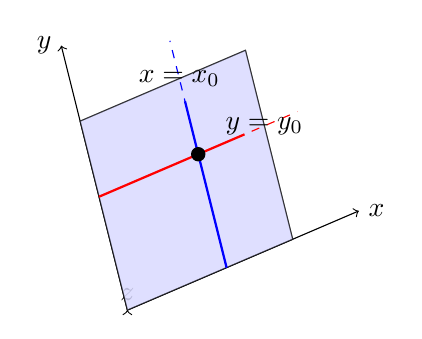
\begin{tikzpicture}[scale=1.2, x={(0.7cm,0.3cm)}, y={(-0.2cm,0.8cm)}, z={(0cm,0cm)}]
    % Ejes
    \draw[->] (0,0,0) -- (3.5,0,0) node[right] {$x$};
    \draw[->] (0,0,0) -- (0,3.5,0) node[left] {$y$};
    \draw[->] (0,0,0) -- (0,0,3.5) node[above] {$z$};
    % Superficie aproximada z = 4 - x^2 - y^2
    \draw[fill=blue!15, opacity=0.6] plot[domain=0:2.5] (\x,0,{4-\x*\x}) -- (2.5,2.5,{4-2.5*2.5-2.5*2.5}) -- (0,2.5,{4-2.5*2.5}) -- cycle;
    \draw[fill=blue!15, opacity=0.6] plot[domain=0:2.5] (0,\x,{4-\x*\x}) -- (2.5,2.5,{4-2.5*2.5-2.5*2.5}) -- (2.5,0,{4-2.5*2.5}) -- cycle;
    % Plano y = y0
    \draw[red, dashed] (0,1.5,0) -- (3,1.5,0);
    \draw[red, dashed] (0,1.5,0) -- (0,1.5,3);
    % Curva en el plano y=y0
    \draw[red, thick] plot[domain=0:2.2] (\x,1.5,{4-\x*\x-2.25});
    % Plano x = x0
    \draw[blue, dashed] (1.5,0,0) -- (1.5,3,0);
    \draw[blue, dashed] (1.5,0,0) -- (1.5,0,3);
    % Curva en el plano x=x0
    \draw[blue, thick] plot[domain=0:2.2] (1.5,\x,{4-2.25-\x*\x});
    % Punto
    \filldraw[black] (1.5,1.5,{4-2.25-2.25}) circle (2pt);
    % Etiquetas
    \node at (2.5,1.5,{4-2.25-6.25}) {$y=y_0$};
    \node at (1.5,2.5,{4-6.25-2.25}) {$x=x_0$};
\end{tikzpicture}
\caption{Interpretación geométrica de las derivadas parciales como
pendientes de tangentes a curvas de intersección con planos
coordenados.}
\end{figure}

% ------------------------------------------------------------
% DERIVADAS PARCIALES DE ORDEN SUPERIOR
% ------------------------------------------------------------

\begin{definition}[Derivadas parciales de segundo orden]
Si $f$ tiene derivadas parciales primeras, podemos derivarlas de
nuevo para obtener las \textbf{derivadas parciales de segundo orden}:
\[
\begin{aligned}
f_{xx} &= \frac{\partial^2 f}{\partial x^2}
       = \frac{\partial}{\partial x}\left(\frac{\partial f}{\partial x}\right),\\
f_{xy} &= \frac{\partial^2 f}{\partial y\partial x}
       = \frac{\partial}{\partial y}\left(\frac{\partial f}{\partial x}\right),\\
f_{yx} &= \frac{\partial^2 f}{\partial x\partial y}
       = \frac{\partial}{\partial x}\left(\frac{\partial f}{\partial y}\right),\\
f_{yy} &= \frac{\partial^2 f}{\partial y^2}
       = \frac{\partial}{\partial y}\left(\frac{\partial f}{\partial y}\right).
\end{aligned}
\]
\end{definition}

\begin{rem}
La notación $f_{xy}$ significa derivar primero respecto a $x$ y
luego respecto a $y$; es decir, $f_{xy}=(f_x)_y$. Algunos autores
escriben $\frac{\partial^2 f}{\partial y\partial x}$ para $f_{xy}$.
\end{rem}

\begin{theorem}[Teorema de Clairaut (igualdad de derivadas cruzadas)]
Si $f$, $f_x$, $f_y$, $f_{xy}$ y $f_{yx}$ son continuas en un disco
abierto que contiene a $(a,b)$, entonces
\[
f_{xy}(a,b) = f_{yx}(a,b).
\]
\end{theorem}

\begin{proof}
La demostración se basa en el Teorema del Valor Medio aplicado a la
función $g(x)=f(x,y+h)-f(x,y)$ y luego a la diferencia en $y$. Bajo
las hipótesis de continuidad, los dos límites que definen $f_{xy}$ y
$f_{yx}$ coinciden. Omitimos los detalles por brevedad.
\end{proof}

\begin{rem}
El Teorema de Clairaut es una gran simplificación: para la mayoría
de las funciones que aparecen en aplicaciones, el orden de derivación
no importa. Esto permite ahorrar trabajo al calcular derivadas
cruzadas: se puede elegir el orden más sencillo.
\end{rem}

\begin{example}[Derivadas parciales de segundo orden]
Calcular todas las derivadas parciales de segundo orden de
$f(x,y)=x^2 e^{xy}$.
\end{example}

\begin{myproof}
\textbf{Paso 1. Primeras derivadas.}
\[
f_x = 2x e^{xy} + x^2 y e^{xy} = (2x + x^2 y)e^{xy},
\]
\[
f_y = x^2 \cdot x e^{xy} = x^3 e^{xy}.
\]

\textbf{Paso 2. Segundas derivadas.}
\[
f_{xx} = \frac{\partial}{\partial x}\left[(2x+x^2y)e^{xy}\right].
\]
Derivamos el producto:
\[
f_{xx} = (2+2xy)e^{xy} + (2x+x^2y)\cdot y e^{xy}
= \bigl[2+2xy + 2xy + x^2 y^2\bigr]e^{xy}
= (2+4xy+x^2 y^2)e^{xy}.
\]

\[
f_{yy} = \frac{\partial}{\partial y}(x^3 e^{xy})
= x^3 \cdot x e^{xy} = x^4 e^{xy}.
\]

\[
f_{xy} = \frac{\partial}{\partial y}(f_x)
= \frac{\partial}{\partial y}\left[(2x+x^2y)e^{xy}\right].
\]
\[
f_{xy} = (x^2)e^{xy} + (2x+x^2y)\cdot x e^{xy}
= (x^2 + 2x^2 + x^3 y)e^{xy}
= (3x^2 + x^3 y)e^{xy}.
\]

\[
f_{yx} = \frac{\partial}{\partial x}(f_y)
= \frac{\partial}{\partial x}(x^3 e^{xy})
= (3x^2 + x^3 y)e^{xy}.
\]

\textbf{Conclusión.}
\[
\boxed{
f_{xx}=(2+4xy+x^2y^2)e^{xy},\quad
f_{yy}=x^4 e^{xy},\quad
f_{xy}=f_{yx}=(3x^2+x^3y)e^{xy}
}
\]
Se verifica $f_{xy}=f_{yx}$.
\end{myproof}

\begin{example}[Derivadas de orden superior]
Calcular $f_{xxx}$ y $f_{xxy}$ para $f(x,y)=\cos(x^2 y)$.
\end{example}

\begin{myproof}
\textbf{Paso 1. Primera derivada respecto a $x$:}
\[
f_x = -\sin(x^2 y)\cdot 2xy = -2xy\sin(x^2 y).
\]

\textbf{Paso 2. Segunda derivada respecto a $x$:}
\[
f_{xx} = \frac{\partial}{\partial x}[-2xy\sin(x^2 y)].
\]
Usamos la regla del producto:
\[
f_{xx} = -2y\sin(x^2 y) - 2xy\cos(x^2 y)\cdot 2xy
= -2y\sin(x^2 y) - 4x^2 y^2 \cos(x^2 y).
\]

\textbf{Paso 3. Tercera derivada respecto a $x$:}
\[
f_{xxx} = \frac{\partial}{\partial x} f_{xx}.
\]
\[
f_{xxx} = -2y\cos(x^2 y)\cdot 2xy
-8xy^2\cos(x^2 y) - 4x^2 y^2(-\sin(x^2 y))\cdot 2xy.
\]
\[
f_{xxx} = -4xy^2\cos(x^2 y) - 8xy^2\cos(x^2 y)
+ 8x^3 y^3 \sin(x^2 y).
\]
\[
\boxed{f_{xxx} = -12xy^2\cos(x^2 y) + 8x^3 y^3 \sin(x^2 y)}
\]

\textbf{Paso 4. Derivada mixta $f_{xxy}$:}
Derivamos $f_{xx}$ respecto a $y$:
\[
f_{xxy} = \frac{\partial}{\partial y}[-2y\sin(x^2 y) - 4x^2 y^2 \cos(x^2 y)].
\]
\[
f_{xxy} = -2\sin(x^2 y) - 2y\cos(x^2 y)\cdot x^2
-8x^2 y\cos(x^2 y) - 4x^2 y^2 (-\sin(x^2 y))\cdot x^2.
\]
\[
\boxed{f_{xxy} = -2\sin(x^2 y) - 2x^2 y\cos(x^2 y)
-8x^2 y\cos(x^2 y) + 4x^4 y^2\sin(x^2 y)}
\]
\[
\boxed{f_{xxy} = -2\sin(x^2 y) -10x^2 y\cos(x^2 y)
+ 4x^4 y^2\sin(x^2 y)}
\]
\end{myproof}

% ------------------------------------------------------------
% EXTENSIÓN A FUNCIONES DE TRES O MÁS VARIABLES
% ------------------------------------------------------------

Para funciones de tres variables $f(x,y,z)$, las derivadas parciales
se definen de manera análoga:
\[
f_x = \lim_{h\to 0}\frac{f(x+h,y,z)-f(x,y,z)}{h},
\]
y de forma similar para $f_y$ y $f_z$. Las derivadas de orden
superior y el Teorema de Clairaut se extienden naturalmente:
$f_{xy}=f_{yx}$, $f_{xz}=f_{zx}$, $f_{yz}=f_{zy}$, siempre que las
derivadas cruzadas sean continuas.

\begin{example}[Derivadas parciales en tres variables]
Calcular $\frac{\partial f}{\partial x}$, $\frac{\partial f}{\partial y}$
y $\frac{\partial f}{\partial z}$ para $f(x,y,z)=e^{xy}\sin z$.
\end{example}

\begin{myproof}
\[
f_x = y e^{xy}\sin z,
\]
\[
f_y = x e^{xy}\sin z,
\]
\[
f_z = e^{xy}\cos z.
\]
$\boxed{f_x=ye^{xy}\sin z,\; f_y=xe^{xy}\sin z,\; f_z=e^{xy}\cos z}$
\end{myproof}

% ------------------------------------------------------------
% IMPORTANCIA DE LAS DERIVADAS PARCIALES
% ------------------------------------------------------------

Las derivadas parciales son el primer paso para entender el
comportamiento local de funciones de varias variables. Permiten:
\begin{itemize}
    \item Calcular planos tangentes y aproximaciones lineales.
    \item Estudiar la variación de una función cuando todas las
    variables cambian simultáneamente (a través del gradiente).
    \item Formular ecuaciones diferenciales parciales, que modelan
    fenómenos como la difusión del calor, el flujo de fluidos o la
    propagación de ondas.
\end{itemize}

\begin{rem}
El Teorema de Clairaut es una herramienta práctica que simplifica el
cálculo: si las derivadas cruzadas son continuas, el orden de
derivación no importa. Esto es especialmente útil cuando una de las
derivadas es mucho más fácil de calcular que la otra.
\end{rem}

% ============================================================
% CONCLUSIÓN
% ============================================================

En esta lección hemos extendido los conceptos fundamentales de
límite, continuidad y derivada al contexto de funciones de varias
variables. La noción de límite adquiere una complejidad nueva: la
existencia del límite exige que el valor límite sea independiente de
la trayectoria de aproximación. La continuidad preserva la idea de
que la gráfica no presenta saltos, y las derivadas parciales permiten
medir cómo cambia la función cuando se varía una variable a la vez.

Estas herramientas son la base para los temas que siguen: el plano
tangente y la aproximación lineal, la regla de la cadena, el
gradiente y las derivadas direccionales, y finalmente la optimización
de funciones de varias variables.

% ============================================================
% PROBLEMAS PROPUESTOS
% ============================================================

\section*{Problemas propuestos}

\subsection*{Límite y continuidad}

\begin{prob}
Calcule los siguientes límites o demuestre que no existen:
\begin{multicols}{2}
\begin{enumerate}
    \item $\displaystyle\lim_{(x,y)\to(0,0)} \frac{x^2 y}{x^2+y^2}$
    \item $\displaystyle\lim_{(x,y)\to(0,0)} \frac{x^4 y^4}{(x^2+y^4)^3}$
    \item $\displaystyle\lim_{(x,y)\to(0,0)} \frac{x^3+y^3}{x^2+y^2}$
    \item $\displaystyle\lim_{(x,y)\to(0,0)} \frac{x^2 y^2}{x^4+y^4}$
    \item $\displaystyle\lim_{(x,y)\to(0,0)} \frac{x^2 y}{x^4+y^2}$
    \item $\displaystyle\lim_{(x,y)\to(0,0)} \frac{\sin(x^2+y^2)}{x^2+y^2}$
    \item $\displaystyle\lim_{(x,y)\to(0,0)} \frac{1-\cos(xy)}{x^2 y^2}$
    \item $\displaystyle\lim_{(x,y)\to(0,0)} \frac{x y}{\sqrt{x^2+y^2}}$
\end{enumerate}
\end{multicols}
\end{prob}

\begin{prob}
Estudie la continuidad de las siguientes funciones en todo su dominio:
\begin{enumerate}
    \item $f(x,y)=\begin{cases}
    \dfrac{x^2-y^2}{x^2+y^2}, & (x,y)\neq(0,0),\\
    0, & (x,y)=(0,0).
    \end{cases}$
    \item $f(x,y)=\begin{cases}
    \dfrac{x^2 y}{x^2+y^2}, & (x,y)\neq(0,0),\\
    0, & (x,y)=(0,0).
    \end{cases}$
    \item $f(x,y)=\begin{cases}
    \dfrac{x^3 y}{x^6+y^2}, & (x,y)\neq(0,0),\\
    0, & (x,y)=(0,0).
    \end{cases}$
\end{enumerate}
\end{prob}

\begin{prob}
Calcule $\displaystyle\lim_{(x,y)\to(0,0)} \frac{x^2+y^2}{\sqrt{x^2+y^2+1}-1}$
usando coordenadas polares.
\end{prob}

\begin{prob}
Demuestre que $\displaystyle\lim_{(x,y)\to(0,0)} \frac{x^2 y^2}{x^2+y^2}=0$
usando el teorema del emparedado.
\end{prob}

\begin{prob}
Sea $f(x,y)=\dfrac{x^3 y}{x^4+y^2}$ para $(x,y)\neq(0,0)$.
\begin{enumerate}
    \item Demuestre que a lo largo de cualquier recta $y=mx$, el límite
    cuando $(x,y)\to(0,0)$ es $0$.
    \item Demuestre que a lo largo de la parábola $y=x^2$, el límite
    es distinto. Concluya que el límite no existe.
\end{enumerate}
\end{prob}

\subsection*{Derivadas parciales}

\begin{prob}
Calcule las primeras derivadas parciales de las siguientes funciones:
\begin{multicols}{2}
\begin{enumerate}
    \item $f(x,y)=x^3-3x^2 y+2y^3$
    \item $f(x,y)=e^{x^2+y^2}$
    \item $f(x,y)=\ln(x^2+y^2+1)$
    \item $f(x,y)=\arctan(y/x)$
    \item $f(x,y)=\sin(x^2 y)$
    \item $f(x,y)=x^y$ ($x>0$)
    \item $f(x,y,z)=x^2 y z^3$
    \item $f(x,y,z)=\ln(x^2+y^2+z^2)$
\end{enumerate}
\end{multicols}
\end{prob}

\begin{prob}
Calcule todas las derivadas parciales de segundo orden de:
\begin{multicols}{2}
\begin{enumerate}
    \item $f(x,y)=x^3 y^2$
    \item $f(x,y)=e^x\cos y$
    \item $f(x,y)=\ln(x^2+y^2)$
    \item $f(x,y)=\sin(x+y)$
\end{enumerate}
\end{multicols}
\end{prob}

\begin{prob}
Verifique el Teorema de Clairaut para $f(x,y)=x^2 e^{xy}$ calculando
$f_{xy}$ y $f_{yx}$.
\end{prob}

\begin{prob}
Calcule $f_{xy}$, $f_{yz}$ y $f_{zx}$ para $f(x,y,z)=x y^2 z^3$.
\end{prob}

\begin{prob}
Sea $f(x,y)=\begin{cases}
\dfrac{x^2 y^2}{x^2+y^2}, & (x,y)\neq(0,0),\\
0, & (x,y)=(0,0).
\end{cases}$
Calcule $f_x(0,0)$ y $f_y(0,0)$ usando la definición.
\end{prob}

\begin{prob}
Demuestre que la función $u(x,t)=\sin(x-at)$ satisface la ecuación de
onda unidimensional $u_{tt}=a^2 u_{xx}$.
\end{prob}

\begin{prob}
Demuestre que $u(x,y)=\ln(x^2+y^2)$ satisface la ecuación de Laplace
$u_{xx}+u_{yy}=0$ para $(x,y)\neq(0,0)$.
\end{prob}

\begin{prob}
Determine si cada afirmación es verdadera o falsa. Justifique.
\begin{enumerate}
    \item Si $\lim_{(x,y)\to(a,b)} f(x,y)$ existe, entonces existe un
    disco abierto centrado en $(a,b)$ donde $f$ está definida.
    \item Si $\lim_{(x,y)\to(a,b)} f(x,y)=L$, entonces
    $\lim_{x\to a} f(x,b)=L$.
    \item Si todos los límites a lo largo de rectas que pasan por
    $(a,b)$ existen y son iguales, entonces el límite existe.
    \item Si $f$ es continua en $(a,b)$, entonces $f_x$ y $f_y$ existen
    en $(a,b)$.
    \item Si $f_x$ y $f_y$ existen en $(a,b)$, entonces $f$ es continua
    en $(a,b)$.
    \item Si $f_{xy}=f_{yx}$ en todo punto, entonces $f$ es continua.
\end{enumerate}
\end{prob}

\begin{prob}
Encuentre los valores de $a$ y $b$ para que la función
\[
f(x,y)=
\begin{cases}
\dfrac{x^a y^b}{x^2+y^2}, & (x,y)\neq(0,0),\\
0, & (x,y)=(0,0)
\end{cases}
\]
sea continua en $(0,0)$.
\end{prob}
\section{Problemas propuestos}


% ============================================================
% Cap. 19 — Límites y continuidad en Rⁿ
% 16 problemas unicos: 16 listos para integrar ahora, 0 esperan pasada Claude Code (pstricks)
% ============================================================

% >>> LISTOS PARA INTEGRAR AHORA <<<

% [Original: líneas 242-259 | solución completa | sin figura]
\begin{prob}
Sea $f(x,y)=\dfrac{x-y}{x+y}.$
\begin{enumerate}[(a)]
    \item Calcule $\displaystyle\lim_{(x,y)\to (0,0)}f(x)$ tomando la trayectoria $y=kx.$
    \item ¿Qué conclusión puede extraer?
\end{enumerate}
\begin{myproof}
Sea $f(x,y)=\dfrac{x-y}{x+y}.$ Observe que:
\begin{enumerate}[$a)$]
\item Tomando la trayectoria $y=kx$ el límite queda así:
\begin{align*}
\displaystyle\lim_{(x,y)\to (0,0)} \dfrac{x-y}{x+y} {{=}\atop {\begin{array}{c}
\uparrow\\ \text{ si $y=kx$}\end{array}} } \displaystyle\lim_{x\to 0}\dfrac{x-kx}{x+kx}=\displaystyle\lim_{x\to 0}\dfrac{x(1-k)}{x(1+k)}=\dfrac{1-k}{1+k}.
\end{align*}
\item El límite no existe, pues depende del valor de $k\in \mathbb{R}$.
\end{enumerate}
\end{myproof}
\end{prob}

% [Original: líneas 285-308 | solución completa | sin figura]
\begin{prob}
Sea $f(x,y)=\dfrac{xy+y^3}{x^2+y^2}.$
\begin{enumerate}[(a)]
    \item Calcule $\displaystyle\lim_{(x,y)\to (0,0)}f(x)$ tomando la trayectoria $y=x.$
    \item Calcule $\displaystyle\lim_{(x,y)\to (0,0)}f(x)$ tomando la trayectoria $y=0.$
    \item ¿Qué conclusión puede extraer?
\end{enumerate}
\begin{myproof}
Sea $f(x,y)=\dfrac{xy+y^3}{x^2+y^2}.$ Observe que:
\begin{enumerate}[$a)$]
\item Tomando la trayectoria $y=x$ el límite queda así:
\begin{align*}
\displaystyle\lim_{(x,y)\to (0,0)} \dfrac{xy+y^3}{x^2+y^2} {{=}\atop {\begin{array}{c}
\uparrow\\ \text{ si $y=x$}\end{array}} } \displaystyle\lim_{x\to 0}\dfrac{x^2+x^3}{x^2+x^2}=\displaystyle\lim_{x\to 0}\dfrac{x^2(1+x)}{2x^2}=\dfrac{1}{2}\lim_{x\to 0}(1+x)=\dfrac{1}{2}.
\end{align*}
\item Tomando la trayectoria $y=0$ el límite queda así:
\begin{align*}
\displaystyle\lim_{(x,y)\to (0,0)} \dfrac{xy+y^3}{x^2+y^2} {{=}\atop {\begin{array}{c}
\uparrow\\ \text{ si $y=0$}\end{array}} } \displaystyle\lim_{x\to 0}\dfrac{x(0)+0^3}{x^2+0^2}=\displaystyle\lim_{x\to 0}\dfrac{0}{x^2}=0.
\end{align*}
\item El límite no existe, pues dos trayectorias determinan un valor distinto.
\end{enumerate}
\end{myproof}
\end{prob}

% [Original: líneas 333-343 | solución completa | sin figura]
\begin{prob}
Sea $f(x,y)=\dfrac{\arctan(xy)}{xy}.$ Sobre esta función se conoce que $1-\dfrac{x^2y^3}{3}<\dfrac{\arctan (xy)}{xy}<1.$ Calcule $\displaystyle\lim_{(x,y)\to (0,0)}f(x,y).$
\begin{myproof}
Sea $f(x,y)=\dfrac{\arctan(xy)}{xy}.$ Observe que:
\begin{enumerate}[$a)$]
\item $\displaystyle\lim_{(x,y)\to (0,0)} 1-\dfrac{x^2y^3}{3} = 1-\displaystyle\lim_{(x,y)\to (0,0)} \dfrac{x^2y^3}{3}=1-0=1.$
\item $\displaystyle\lim_{(x,y)\to (0,0)} 1=1.$
\item Por medio del teorema del emparedado el límite de la función $f(x,y)=\dfrac{\arctan(xy)}{xy}$  existe y es igual a $1.$
\end{enumerate}
\end{myproof}
\end{prob}

% [Original: líneas 429-446 | solución completa | sin figura]
\begin{prob}
Sea $f(x,y)=\dfrac{x^4y}{x^8+y^2}.$
\begin{enumerate}[(a)]
    \item Determine los puntos donde la función es discontinua.
    \item Exprese si es posible remover las discontinuidades encontradas en el primer punto. Si lo es, determine los valores que hacen que la función sea continua. 
\end{enumerate}
\begin{myproof}
\begin{enumerate}[(a)]
\item Observe que la función solo se indetermina cuando $x^8+y^2=0,$ lo cual ocurre cuando $(x,y)=(0,0).$ De esta manera, al calcular el límite:
 \begin{align*}
\displaystyle\lim_{(x,y)\to (0,0)} \dfrac{x^4y}{x^8+y^2} {{=}\atop {\begin{array}{c}
\uparrow\\ \text{ si $y=mx^4$}\end{array}} } \displaystyle\lim_{x\to 0}\dfrac{x^4mx^4}{x^8+(mx^4)^2}=\displaystyle\lim_{x\to 0}\dfrac{x^8(m)}{x^8(1+m^2)}=\displaystyle\dfrac{m}{1+m^2}.
\end{align*}
Como este límite depende de $m,$ no existe.
\item No es posible remover las discontinuidades, pues el límite cuando la función tiende a $(0,0)$ no existe.
\end{enumerate}
\end{myproof}
\end{prob}

% [Original: líneas 685-702 | solución completa | sin figura]
\begin{prob}
Sea $f(x,y)=\dfrac{2xy^4}{x^5+6y^5}.$
\begin{enumerate}[(a)]
    \item Determine los puntos donde la función es discontinua.
    \item Exprese si es posible remover las discontinuidades encontradas en el primer punto. Si lo es, determine los valores que hacen que la función sea continua. 
\end{enumerate}
\begin{myproof}
\begin{enumerate}[(a)]
\item Observe que la función solo se indetermina cuando $x^5+6y^5=0,$ lo cual ocurre cuando $(x,y)=(0,0).$ De esta manera, al calcular el límite:
 \begin{align*}
\displaystyle\lim_{(x,y)\to (0,0)} \dfrac{2xy^4}{x^5+6y^5} {{=}\atop {\begin{array}{c}
\uparrow\\ \text{ si $y=mx$}\end{array}} } \displaystyle\lim_{x\to 0}\dfrac{2xm^4x^4}{x^5+6(mx)^5}=\displaystyle\lim_{x\to 0}\dfrac{x^5(2m^4)}{x^5(1+6m^5)}=\displaystyle\dfrac{2m^4}{1+6m^5}.
\end{align*}
Como este límite depende de $m,$ no existe.
\item No es posible remover las discontinuidades, pues el límite cuando la función tiende a $(0,0)$ no existe.
\end{enumerate}
\end{myproof}
\end{prob}

% [Original: líneas 847-863 | solución completa | sin figura]
\begin{prob}
Sea $f(x,y)=\dfrac{8x^3y^2}{x^9+y^3}.$
\begin{enumerate}[(a)]
    \item Determine los puntos donde la función es discontinua.
    \item Exprese si es posible remover las discontinuidades encontradas en el primer punto. Si lo es, determine los valores que hacen que la función sea continua. 
\end{enumerate}
\begin{myproof}
\begin{enumerate}[(a)]
\item Observe que la función solo se indetermina cuando $x^9+y^3=0,$ lo cual ocurre cuando $y=-x^3.$ Suponga así que  $x=k$ entonces $y=-k^3.$ Así, al calcular el límite:
 \begin{align*}
\displaystyle\lim_{(x,y)\to (k,-k^3)} \dfrac{8x^3y^2}{x^9+y^3} = \displaystyle\lim_{x\to k}\dfrac{8k^3(-k^3)^2}{k^9+(-k^3)^3}&=\displaystyle\lim_{x\to k}\dfrac{8k^3(k^6)}{k^9+(-k^3)^3}\\&=\displaystyle\lim_{x\to k}\dfrac{8k^9}{k^9-k^9}=\displaystyle\dfrac{8k^9}{0}.
\end{align*}
El cual es un límite que no existe.
\item No es posible remover las discontinuidades sobre $y=-x^3$, pues el límite sobre los puntos de esta curva no existe.
\end{enumerate}
\end{myproof}
\end{prob}

% [Original: líneas 921-923 | sin verificar | sin figura]
\begin{prob}
Calcule $\displaystyle\lim_{(x,y)\to (0,0)}\left(\dfrac{x^4y^2+x^2y^4-5x^2-5y^2}{x^2+y^2}\right).$
\end{prob}

% [Original: líneas 945-947 | sin verificar | sin figura | 2 variante(s) de parámetro (se descartaron 1)]
\begin{prob}
Calcule $\displaystyle\lim_{(x,y)\to (5,9)}xy^2\left(\dfrac{x+4y}{x-y}\right).$
\end{prob}

% [Original: líneas 961-963 | sin verificar | sin figura]
\begin{prob}
Calcule $\displaystyle\lim_{(x,y)\to (2,1)}\ln\left(2x^2-3y^2\right).$
\end{prob}

% [Original: líneas 1020-1037 | solución completa | sin figura]
\begin{prob}
Sea $f(x,y)=\dfrac{x+y}{x-y}.$
\begin{enumerate}[(a)]
    \item Calcule $\displaystyle\lim_{(x,y)\to (0,0)}f(x)$ tomando la trayectoria $y=mx.$
    \item ¿Qué conclusión puede extraer?
\end{enumerate}
\begin{myproof}
Sea $f(x,y)=\dfrac{x+y}{x-y}.$ Observe que:
\begin{enumerate}[$a)$]
\item Tomando la trayectoria $y=mx$ el límite queda así:
\begin{align*}
\displaystyle\lim_{(x,y)\to (0,0)} \dfrac{x+y}{x-y} {{=}\atop {\begin{array}{c}
\uparrow\\ \text{ si $y=mx$}\end{array}} } \displaystyle\lim_{x\to 0}\dfrac{x+kx}{x-kx}=\displaystyle\lim_{x\to 0}\dfrac{x(1+k)}{x(1-k)}=\dfrac{1+k}{1-k}.
\end{align*}
\item El límite no existe, pues depende del valor de $k\in \mathbb{R}$.
\end{enumerate}
\end{myproof}
\end{prob}

% [Original: líneas 1063-1086 | solución completa | sin figura]
\begin{prob}
Sea $f(x,y)=\dfrac{x^4-y^2}{x^4+y^2}.$
\begin{enumerate}[(a)]
    \item Calcule $\displaystyle\lim_{(x,y)\to (0,0)}f(x)$ tomando la trayectoria $y=mx^2.$
    \item Calcule $\displaystyle\lim_{(x,y)\to (0,0)}f(x)$ tomando la trayectoria $y=0.$
    \item ¿Qué conclusión puede extraer?
\end{enumerate}
\begin{myproof}
Sea $f(x,y)=\dfrac{x^4-y^2}{x^4+y^2}.$ Observe que:
\begin{enumerate}[$a)$]
\item Tomando la trayectoria $y=mx^2$ el límite queda así:
\begin{align*}
\displaystyle\lim_{(x,y)\to (0,0)} \dfrac{x^4-y^2}{x^4+y^2} &{{=}\atop {\begin{array}{c}
\uparrow\\ \text{ si $y=mx^2$}\end{array}} } \displaystyle\lim_{x\to 0}\dfrac{x^4-m^2x^4}{x^4+m^2x^4}=\displaystyle\lim_{x\to 0}\dfrac{x^4(1-m^2)}{1+m^2}\\&=\lim_{x\to 0}\dfrac{1-m^2}{1+m^2}=\dfrac{1-m^2}{1+m^2}.
\end{align*}
\item Tomando la trayectoria $y=0$ el límite queda así:
\begin{align*}
\displaystyle\lim_{(x,y)\to (0,0)} \dfrac{x^4-y^2}{x^4+y^2} {{=}\atop {\begin{array}{c}
\uparrow\\ \text{ si $y=0$}\end{array}} } \displaystyle\lim_{x\to 0}\dfrac{x^4}{x^4}=1.
\end{align*}
\item El límite no existe, pues dos trayectorias determinan un valor distinto.
\end{enumerate}
\end{myproof}
\end{prob}

% [Original: líneas 1111-1121 | solución completa | sin figura]
\begin{prob}
Sea $f(x,y)=x\cos\left(\dfrac{1}{y}\right).$ Sobre esta función se conoce que $-1\leq \cos\left(\dfrac{1}{y}\right)\leq 1$ Calcule $\displaystyle\lim_{(x,y)\to (0,0)}f(x,y).$
\begin{myproof}
Sea $f(x,y)=x\cos\left(\dfrac{1}{y}\right).$ Observe que:
\begin{enumerate}[$a)$]
\item $\displaystyle\lim_{(x,y)\to (0,0)} x = 0.$
\item $\displaystyle\lim_{(x,y)\to (0,0)} -x = 0.$
\item Por medio del teorema del emparedado el límite de la función $f(x,y)=x\cos\left(\dfrac{1}{y}\right)$  existe y es igual a $0.$
\end{enumerate}
\end{myproof}
\end{prob}

% [Original: líneas 1147-1154 | sin verificar | sin figura]
\begin{prob}
Dada la función $f(x,y)=\dfrac{x^3+y^3}{x^2+y^2}$ determine:
\begin{parts}
\part El dominio de la función.
\part De acuerdo al resultado obtenido en el anterior ítem, ¿es posible redefinir la función $f(x,y)$ para que sea continua en todo $\mathbb{R}^2$?
\textit{Sugerencia:} Considere hacer una división de polinomios.
\end{parts}
\end{prob}

% [Original: líneas 1248-1250 | sin verificar | sin figura]
\begin{prob}
Determine si $\displaystyle\lim_{(x,y)\to (0,0)} \dfrac{Axy}{x^2+y^2}$ existe. Justifique adecuadamente su respuesta.
\end{prob}

% [Original: líneas 1380-1382 | sin verificar | sin figura]
\begin{prob}
Calcule $\displaystyle\lim_{(x,y)\to (0,0)}\left(\dfrac{x^3y+xy^3-3x^2-3y^2}{x^2+y^2}\right).$
\end{prob}

% [Original: líneas 1420-1422 | sin verificar | sin figura]
\begin{prob}
Calcule $\displaystyle\lim_{(x,y)\to (1,1)}\ln\left(2x^2-y^2\right).$
\end{prob}


